\documentclass[../../main.tex]{subfiles}
\graphicspath{{\subfix{../../images/}}}

\begin{document}
Gegeben ist folgende Linie mit folgenden Punkten:
$P_1 = (2, 3, 0)$
$P_2 = (8, 5, 0)$ \\
Drehe die Line mithilfe einer Matrix um 180 Grad um die X-Achse.


\begin{figure}[h]
    \centering
    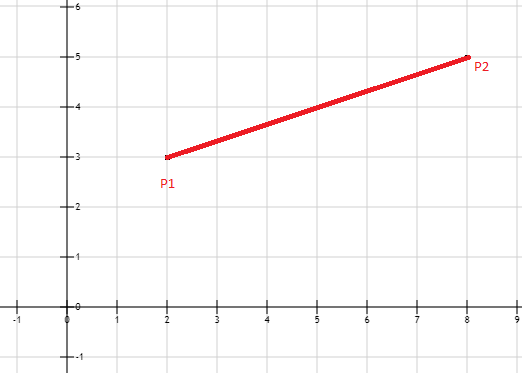
\includegraphics[width=0.75\textwidth]{rotation}
    \caption{Die zu drehende Linie}
    \label{fig:rotation}
\end{figure}



\end{document}